% \documentclass[tikz,border=3.14mm]{standalone}
\documentclass[12pt]{standalone}
\usepackage{polyglossia}
\setdefaultlanguage{vietnamese}
\setotherlanguages{english}
\usepackage{fontspec}
\usepackage{
    amsmath, 
    amsfonts, 
    amssymb
}
\usepackage{unicode-math}
\setmainfont{STIX Two Text}
\setmathfont{STIX Two Math} 
\usepackage{tikz}
\usepackage{amsmath}

\begin{document}

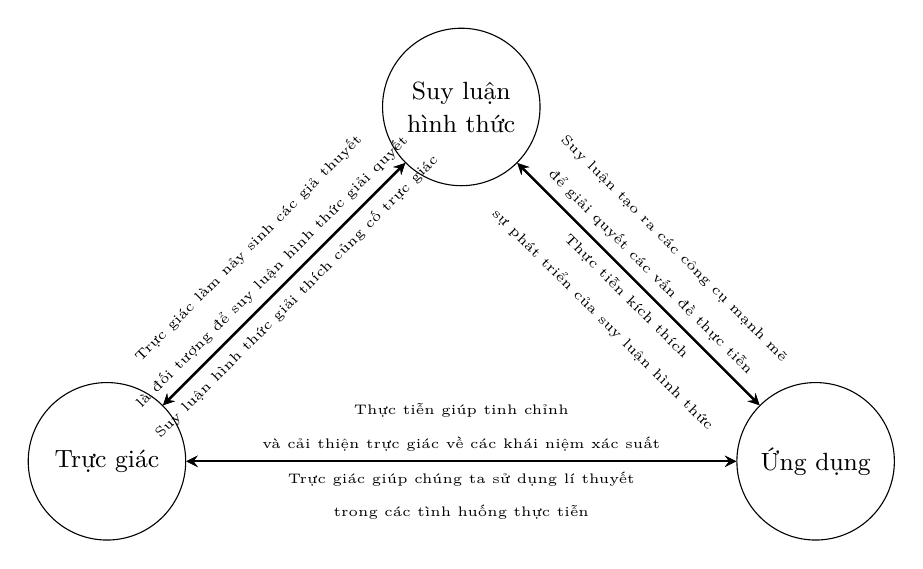
\begin{tikzpicture}[scale=3, every node/.style={scale=1}, >=stealth]

    % Đỉnh của tam giác với các hình tròn bao quanh
    \node[draw, circle, minimum size=2cm, align=center] (A) at (0,1.5) {\small Suy luận\\ \small hình thức};
    \node[draw, circle, minimum size=2cm, align=center] (B) at (-1.5,0) {\small Trực giác};
\node[draw, circle, minimum size=2cm, align=center] (C) at (1.5,0) {\small Ứng dụng};
    
    % Vẽ các cạnh của tam giác với mũi tên hai đầu
    \draw[<->, thick, above] (A) -- (B) node[midway, above, sloped, align=center] {\tiny Trực giác làm nảy sinh các giả thuyết \\ \tiny là đối tượng để suy luận hình thức giải quyết};
    \draw[<->, thick, above] (A) -- (B) node[midway, below, sloped, align=center] {\tiny Suy luận hình thức giải thích củng cố trực giác};

    \draw[<->, thick] (C) -- (A) node[midway, above, sloped, align=center] {\tiny Suy luận tạo ra các công cụ mạnh mẽ \\ \tiny để giải quyết các vấn đề thực tiễn};
    \draw[<->, thick] (C) -- (A) node[midway, below, sloped, align=center] {\tiny Thực tiễn kích thích \\ \tiny sự phát triển của suy luận hình thức};

    
    \draw[<->, thick] (B) -- (C) node[midway, below, align=center] {\tiny Trực giác giúp chúng ta sử dụng lí thuyết \\ \tiny trong các tình huống thực tiễn};
    \draw[<->, thick] (B) -- (C) node[midway, above, align=center] {\tiny Thực tiễn giúp tinh chỉnh \\ \tiny và cải thiện trực giác về các khái niệm xác suất};

    
\end{tikzpicture}

\end{document}

